\documentclass[12pt, a4paper]{article} %determina o tamanho da fonte, o tipo de papel e o tipo de documento.

\setlength{\parindent}{1.0 cm} %tamanho do espaço para começar o parágrafo.
\setlength{\parskip}{0.5cm} %tamanho do espaço entre os parágrafos.

%Aqui ficam os pacotes utilizados para formatação do documento de modo geral:

\usepackage[utf8]{inputenc} 
\usepackage{indentfirst} %Coloca espaços nos inícios de parágrafos automaticamente. 
\usepackage[brazilian]{babel} %
\usepackage{amsmath}
\usepackage[hmargin=3cm, vmargin=2.5cm, bmargin=2.5cm]{geometry}
\usepackage{multicol}
\usepackage{graphicx} %para poder inserir imagens
\usepackage{subfig}
\usepackage{booktabs} 
\usepackage{hyperref} %para poder adicionar links e hiperlinks
\usepackage{float} %para poder posicionar as imagens


\usepackage{listings} %para poder incluir códigos
\usepackage{xcolor}
\definecolor{codegreen}{rgb}{0,0.6,0}
\definecolor{codegray}{rgb}{0.5,0.5,0.5}
\definecolor{codepurple}{rgb}{0.58,0,0.82}
\definecolor{backcolour}{rgb}{0.95,0.95,0.92}

\begin{document} %começa alguma coisa,neste caso, o documento, sempre importante lembrar de colocar o \end{} para não dar erro 
	
	\begin{titlepage}
		\begin{center}
\Huge{Universidade de São Paulo}\\
\large{Instituto de Física de São Carlos}\\
\vspace{20pt}
\vspace{200pt}
\textbf{Notas de Aula C\'alculo 0: Revis\~ao P1 de F\'isica I}\\
\vspace{2cm}
Pedro Calligaris Delbem\\
\end{center}

		\begin{center}
			\vspace{\fill}
	Abril de 2025	
		\end{center}
	\end{titlepage}

%####################################################################### SUMÁRIO
	\tableofcontents 
	\thispagestyle{empty}
	\newpage
%#########################################################################


\section{Exerc\'icio 1}
{        Um rio tem largura $L=0.76Km$ e uma correnteza, paralela \'a margem, com velocidade de $v_{corr}=4km/h$. Um barco tem rapidez m\'axima de $v_{barco}=4m/s$ em \'aguas paradas. Determine o \^angulo de inclina\c{c}\~ao do barco em rela\c{c}\~ao ao rio para que o mesmo atravesse o rio em linha reta.

    \textbf{Desenhando:}

    \begin{figure}[H]
        \centering
        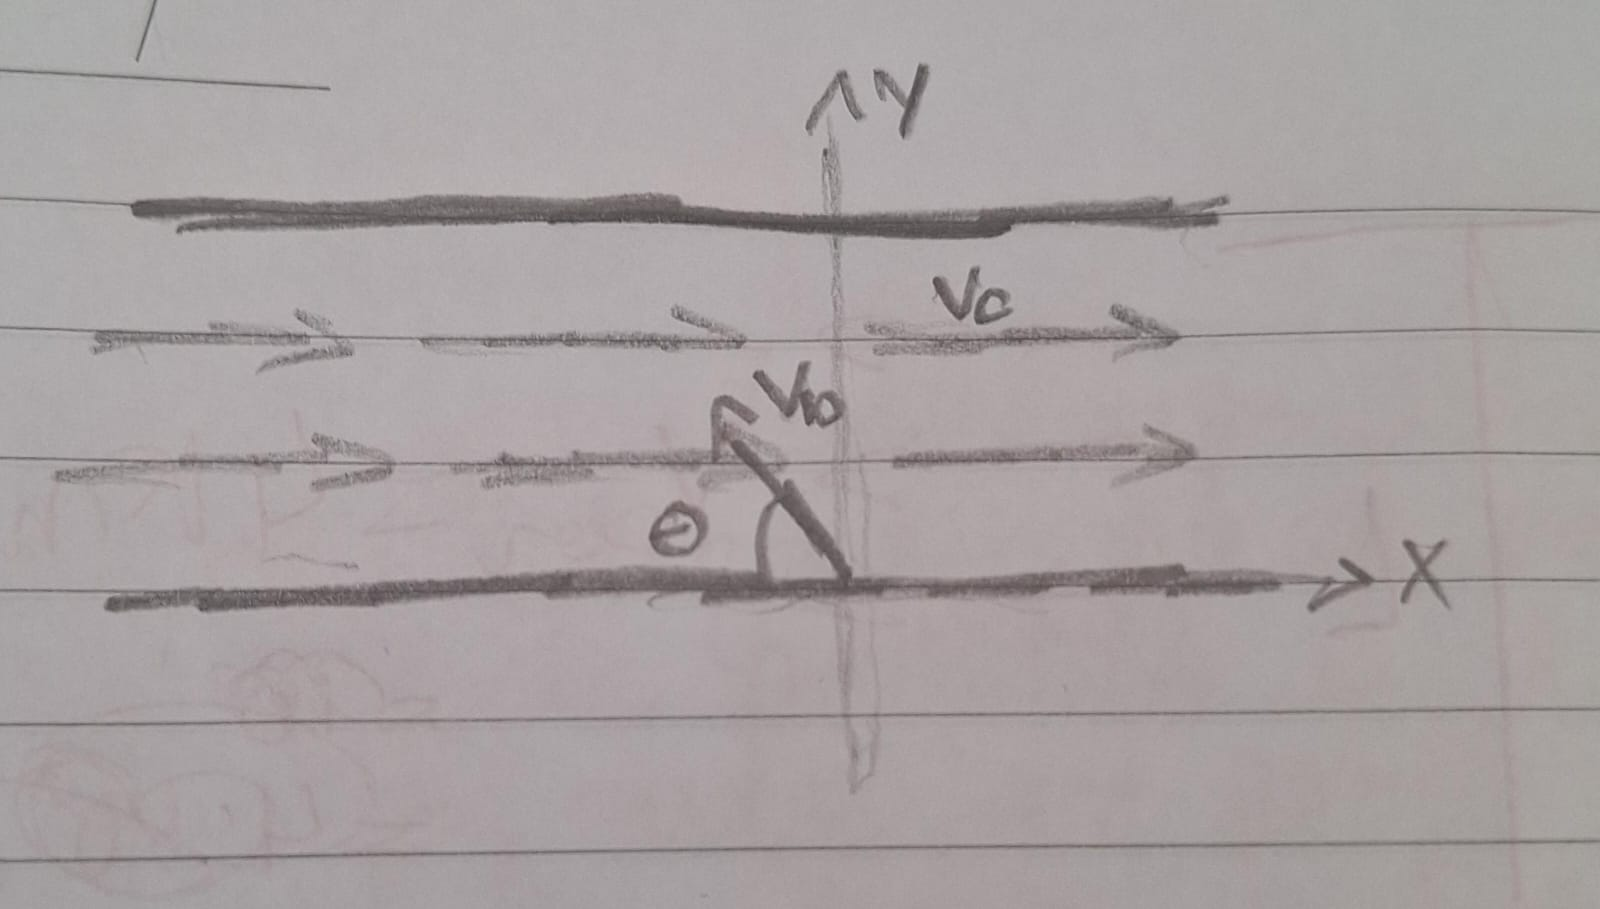
\includegraphics[width=0.5\textwidth]{imagens/ex1.jpeg}
        \caption{Desenho do exerc\'icio 1}
        \label{fig:ex1}
        
    \end{figure}

    \textbf{Solu\c{c}\~ao:}

    Decompor a velocidade do barco em duas componentes: uma na dire\c{c}\~ao do rio e outra na dire\c{c}\~ao perpendicular ao rio.
    \begin{equation}
        \overrightarrow{v_{b}}  = v_{b}\cos\theta \hat{x} + v_{b}\sin\theta \hat{y} 
    \end{equation}
    A componente na dire\c{c}\~ao do rio deve ser igual a velocidade da correnteza para que o barco tenha velocidade nula na dire\c{c}\~ao da correteza do rio, ou seja:
    \begin{equation}
        v_{b}\cos\theta = v_{c}
    \end{equation}
    Isolando para $\theta$:
    \begin{equation}
        \theta = \arccos\left(\frac{v_{c}}{v_{b}}\right)
    \end{equation}
    Numericamente:
    \begin{equation}
        \theta = \arccos\left(\frac{1.11}{4}\right) \approx 73.87^{\circ}
    \end{equation}}


    
\section{Exerc\'icio 2}
    Uma part\'icula tem um vetor posi\c{c}\~ao dado por $\overrightarrow{r} = 30t \hat{i} + (40t - 5t^{2}) \hat{j}$ onde t est\'a em segundos e $\overrightarrow{r}$ em metros. Determine a velocidade e a acelera\c{c}\~ao da part\'icula em um instante t qualquer.

    \textbf{Solu\c{c}\~ao:}
    A velocidade para um instante t qualquer ser\'a dada pela derivada do vetor posi\c{c}\~ao em rela\c{c}\~ao ao tempo:
    \begin{equation}
        \overrightarrow{v} = \frac{d\overrightarrow{r}}{dt} = \frac{d}{dt}(30t \hat{i} + (40t - 5t^{2}) \hat{j}) = 30\hat{i} + (40 - 10t)\hat{j}
    \end{equation}
    A acelera\c{c}\~ao para um instante t qualquer ser\'a dada pela derivada do vetor velocidade em rela\c{c}\~ao ao tempo:
    \begin{equation}
        \overrightarrow{a} = \frac{d\overrightarrow{v}}{dt} = \frac{d}{dt}(30\hat{i} + (40 - 10t)\hat{j}) = -10\hat{j}
    \end{equation}

\section{Exerc\'icio 3}
    A Terra gira em torno de seu eixo uma vez a cada 24 horas, de forma que os objetos em sua superf\'icie executam movimento circular uniforme em torno do eixo com um per\'iodo de 24 horas. Considere apenas o efeito desta rota\c{c}\~ao sobre uma pessoa na superf\'icie. (Ignore o movimento orbital da Terra em torno do Sol.)
    
    (a) Qual \'e a rapidez, e qual \'e a magnitude da acelera\c{c}\~ao de uma pessoa no equador? (Expresse a magnitude desta acelera\c{c}\~ao como uma porcentagem de g.)

    \textbf{Solu\c{c}\~ao:}
    Primeiro obtemos a velocidade angular em fun\c{c}\~ao do per\'iodo:
    \begin{equation}
        \omega = \frac{2\pi}{T}
    \end{equation}
    Onde T \'e o per\'iodo de rota\c{c}\~ao da Terra, que \'e de 24 horas ou $86400s$.
    A velocidade linear \'e dada por:
    \begin{equation}
        v = \omega r
    \end{equation}
    Onde r \'e o raio da Terra, que \'e de aproximadamente $6.37 \times 10^{6}m$.
    Assim, a velocidade linear \'e dada por:
    \begin{equation}
        v = \frac{2\pi r}{T} = \frac{2\pi (6.37 \times 10^{6})}{86400} \approx 465.1 m/s
    \end{equation}
    A acelera\c{c}\~ao centr\'ipeta \'e dada por:
    \begin{equation}
        a = \frac{v^{2}}{r} = \frac{(465.1)^{2}}{6.37 \times 10^{6}} \approx 0.034 m/s^{2}
    \end{equation}
    Em forma percentual, a acelera\c{c}\~ao centr\'ipeta \'e dada por:
    \begin{equation}
        a = \frac{0.034}{9.81} \approx 0.0035 \approx 0.35\%
    \end{equation}
    
    (b) Qual \'e a orienta\c{c}\~ao do vetor acelera\c{c}\~a?

    \textbf{Solu\c{c}\~ao:}
    O vetor acelera\c{c}\~ao \'e perpendicular ao vetor velocidade que est\'a na dire\c{c}\~ao do movimento circular. Assim, o vetor acelera\c{c}\~ao \'e radial e aponta para o centro da Terra.
    Assim, o vetor acelera\c{c}\~ao \'e dado por:
    \begin{equation}
        \overrightarrow{a} = -\frac{v^{2}}{r}\hat{r}
    \end{equation}
    Onde $\hat{r}$ \'e o vetor unit\'ario radial que aponta para fora da Terra.
    
    (c) Qual \'e a rapidez e qual \'e a magnitude da acelera\c{c}\~ao de uma pessoa na superf\'icie, a $35^{\circ}$ de latitude norte?
    
    \textbf{Solu\c{c}\~ao:}
    Primeiro obtemos a velocidade angular em fun\c{c}\~ao do per\'iodo:
    \begin{equation}
        \omega = \frac{2\pi}{T}
    \end{equation}
    Onde T \'e o per\'iodo de rota\c{c}\~ao da Terra, que \'e de 24 horas ou $86400s$.
    A velocidade linear \'e dada por:
    \begin{equation}
        v = \omega r
    \end{equation}
    Onde r \'e o raio da Terra a $35^{\circ}$ de latitude norte que tem um valor de $6.37 \times 10^{6} \cos(35^{\circ})$.
    Assim, a velocidade linear \'e dada por:
    \begin{equation}
        v = \frac{2\pi r}{T} = \frac{2\pi (6.37 \times 10^{6} \cos(35^{\circ}))}{86400} \approx 380.1 m/s
    \end{equation}
    A acelera\c{c}\~ao centr\'ipeta \'e dada por:
    \begin{equation}
        a = \frac{v^{2}}{r} = \frac{(465.1)^{2}}{6.37 \times 10^{6} \cos(35^{\circ})} \approx 0.042 m/s^{2}
    \end{equation}
    
    (d) Qual \'e o \^angulo entre o sentido da acelera\c{c}\~ao da pessoa a $35^{\circ}$ de latitude norte e o sentido da acelera\c{c}\~ao da pessoa no equador, se as duas pessoas est\~ao em uma mesma longitude?

    Ambos os vetores acelera\c{c}\~ao est\~ao na mesma dire\c{c}\~ao, ou seja, ambos os vetores acelera\c{c}\~ao est\~ao apontando para o centro da Terra. Assim, o \^angulo entre os dois vetores acelera\c{c}\~ao \'e de $0^{\circ}$.


\section{Exerc\'icio 4}
    Na figura abaixo, qual \'e a rapidez inicial m\'inima que o dardo deve ter para atingir o macaco antes que este chegue ao ch\~ao, que est\'a 11,2 m abaixo da posi\c{c}\~ao inicial do macaco, se x = 50 me 10 m? (Ignore a resistência do ar.)

    \begin{center}
        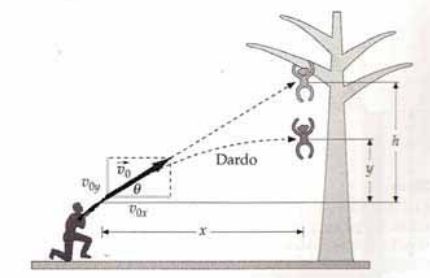
\includegraphics[scale=0.5]{imagens/ex4.png}
    \end{center}
    \textbf{Solu\c{c}\~ao:}
    Vamos escrever a terceira lei de Newton para o macaco:
    \begin{equation}
        \overrightarrow{F_{m}} = m_{m}\overrightarrow{a_{m}} = -m_{m}g\hat{j}
    \end{equation}
    E como a acelera\c{c}\~ao do macaco \'e a segunda derivada da posi\c{c}\~ao do macaco, podemos escrever:
    \begin{equation}
        m_{m}\frac{d^{2}\overrightarrow{r_{m}}}{dt^{2}} = -m_{m}g\hat{j}
    \end{equation}
    Como a acerela\c{c}\~ao est\'a apenas na dire\c{c}\~ao do eixo $j$, podemos escrever:
    \begin{equation}
        \frac{d^{2}y_{m}}{dt^{2}} = -g
    \end{equation}
    Integramos duas vezes para obter a posi\c{c}\~ao do macaco em fun\c{c}\~ao do tempo - utilizando a regra $$\int x^{n}dx = \frac{x^{n+1}}{n+1} + C$$ - e obtemos:
    \begin{equation}
        y_{m} = \frac{1}{2}gt^{2} + v_{y_{m_{0}}}t + y_{m_{0}}
    \end{equation}
    Onde $v_{y_{m_{0}}}$ \'e a velocidade inicial do macaco (que \'e zero) e $y_{m_{0}}$ \'e a posi\c{c}\~ao inicial do macaco que \'e 11,2 m.
    Com o mesmo procedimento para o dardo, obtemos:
    \begin{equation}
        y_{d} = \frac{1}{2}gt^{2} + v_{y_{d_{0}}}t + y_{d_{0}}
    \end{equation}
    Onde $v_{y_{d_{0}}}$ \'e a velocidade inicial do dardo na dire\c{c}\~ao vertical e $y_{d_{0}}$ \'e a posi\c{c}\~ao inicial do dardo que \'e 11,2 m.
    \begin{equation}
        x_{d} = v_{x_{d_{0}}}t + x_{d_{0}}
    \end{equation}
    Onde $v_{x_{d_{0}}}$ \'e a rapidez inicial do dardo na dire\c{c}\~ao horizontal e $x_{d_{0}}$ \'e a posi\c{c}\~ao inicial do dardo que \'e nula.

    O dardo precisa estar na mesma posi\c{c}\~ao horizontal do macaco para atingi-lo. Assim, temos:
    \begin{equation}
        x_{d} = x_{m} = 50
    \end{equation}
    O que nos leva ao instante de tempo da colis\~ao:
    \begin{equation}
        t = \frac{50}{v_{x_{d_{0}}}}
    \end{equation}
    Al\'em disso a altura do dardo deve ser igual a altura do macaco. Assim, temos:
    \begin{equation}
        y_{d} = y_{m}
    \end{equation}
    Ou seja:
    \begin{equation}
        \frac{1}{2}gt^{2} + y_{m_{0}} = y_{d} = \frac{1}{2}gt^{2} + v_{y_{d_{0}}}t + y_{d_{0}}
    \end{equation}
    Logo:
    \begin{equation}
        y_{m_{0}} = v_{y_{d_{0}}}t + y_{d_{0}}
    \end{equation}
    Ou seja:
    \begin{equation}
        v_{y_{d_{0}}}t = y_{m_{0}} - y_{d_{0}} = 1.2m
    \end{equation}
    Utilizando a equa\c{c}\~ao 24:
    \begin{equation}
        \frac{v_{y_{d_{0}}}50}{v_{x_{d_{0}}}} = 1.2m
    \end{equation}
    E como $v_{x_{d_{0}}}$ e $v_{y_{d_{0}}}$ s\~ao dados por:
    \begin{equation}
        v_{x_{d_{0}}} v_{d_{0}} cos\theta
    \end{equation}
    \begin{equation}
        v_{y_{d_{0}}} v_{d_{0}} sin\theta
    \end{equation}
    Logo:
    \begin{equation}
        50 tan\theta = 1.2
    \end{equation}
    Ou seja:
    \begin{equation}
        tan\theta = \frac{1.2m}{50} = 0.02
    \end{equation}
    A velocidade m\'inima ser\'a aquela para qual o macaco praticamente chega ao ch\~ao. Assim, temos:
    \begin{equation}
        \frac{1}{2}g{t_{f}}^{2} + y_{m_{0}} = 0
    \end{equation}
    Ou seja o tempo final \'e:
    \begin{equation}
        t_{f} = \sqrt{\frac{2y_{m_{0}}}{g}}
    \end{equation}
    Substituindo na equa\c{c}\~ao 24:
    \begin{equation}
        t_{f} = \frac{50}{v_{d_{0}}cos\theta}
    \end{equation}
    Resolvendo para $v_{d_{0}}$:
    \begin{equation}
        v_{d_{0}} = \frac{50}{t_{f}cos\theta}
    \end{equation}
    Por fim:
    \begin{equation}
        v_{d_{0}} \approx 33.095 m/s
    \end{equation}

\section{Exerc\'icio 5}
    0 dispositivo da figura gira em torno do eixo vertical com a velocidade angular $\omega$.
    
    (a) Qual deve ser o valor de o para que o fio de comprimento l com a bolinha suspensa de massa m fa\c{c}a um \^angulo e com a vertical?
    
    \textbf{Solu\c{c}\~ao:}
    Como a bolinha \'e suspensa, não temos movimento no plano do desenho - assim a soma das forças em x e y devem ser zero:
    \begin{equation}
        Tcos\theta - mg = 0
    \end{equation}
    E tamb\'em:
    \begin{equation}
        Tsin\theta - ma_{cp} = 0
    \end{equation}
    Logo:
    \begin{equation}
        Tcos\theta = mg
    \end{equation}
    \begin{equation}
        Tsin\theta = ma_{cp}
    \end{equation}
    E sabemo que a acelera\c{c}\~ao centr\'ipeta \'e:
    \begin{equation}
        a_{cp} = \frac{v^2}{r}
    \end{equation}
    Onde
    \begin{equation}
        v = \omega r
    \end{equation}
    Logo:
    \begin{equation}
        a_{cp} = \omega^2 r
    \end{equation}
    E temos que $r=d+lsin\theta$
    Logo:
    \begin{equation}
        a_{cp} = \omega^2 (d+lsin\theta)
    \end{equation}
    Substituimos isto na equa\c{c}\~ao 42 e fazemos a divis\~ao da equa\c{c}\~ao 42 pela equa\c{c}\~ao 41:
    \begin{equation}
        tan\theta = \frac{\omega^2 (d+lsin\theta)}{g}
    \end{equation}
    Isolando para $\omega$:
    \begin{equation}
        \omega = \sqrt{\frac{g tan\theta}{d+lsin\theta}}
    \end{equation}

    (b) Qual \'e a tens\~ao T no fio nessa situa\c{c}\~ao?
    
    \textbf{Solu\c{c}\~ao:}
    Substituindo a equa\c{c}\~ao 48 na equa\c{c}\~ao 42:
    \begin{equation}
        T = mgsec\theta
    \end{equation}


       
\end{document}